\documentclass[12pt]{article}
\usepackage{verbatim,graphicx}
\usepackage{hyperref}
\usepackage{multicol}

\oddsidemargin 5mm
\topmargin -21mm
\textwidth 162mm
\textheight 225mm
\headsep 20mm

\title{
           Hugh Murrell \\
           Resume \\
       }
\date{April 2021}
\begin{document}

\maketitle


%\begin{figure}[ht]
%\center{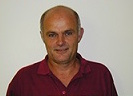
\includegraphics[scale=1.0,clip]{HughMurrell.jpg}}
%\end{figure}
%\begin{flushright}
%\vspace{1.5cm}
%Mbona Private Nature Reserve \\
%Karkloof, KwaZulu-Natal \\
%South Africa \\
%\vspace{0.5cm}
%retired Prof of Computer Science \\ 
%University of KwaZulu-Natal \\
%
%\end{flushright}

%\newpage
\small

\begin{multicols}{2}
\begin{description}\item[] \begin{description}\item[] {\large \bf   Personal Details  }
\item[Address]  Site H13, Mbona Mountain Estate, Karkloof, South Africa.
\item[Postal Address] PO Box 895, Howick, KwaZulu-Natal, SouthAfrica.
\item[e-mail]  \url{hugh.murrell@gmail.com}
\item[url]  \url{http://hughmurrell.github.io}
\item[Phone]  +2776 6864721 (cell) 
\item[Birth Date]  17 December 1954.
\item[Birth Place]  Kasama, Zambia.
\item[Citizenship]  dual, South African and British
\end{description}
\end{description}

\begin{description}\item[] \begin{description}\item[] {\large \bf   Education  }    
\item[1971:] Matric, Hyde Park, Johannesburg.
  \item[1975:]  B.Sc., Natal University, Pietermaritzburg. 
  \item[1981:]  B.Sc. Hons, Rhodes University, Grahamstown. 
  \item[1982: ] M.Sc., Rhodes University, Grahamstown. 
  \item[1995: ] PhD., Natal University, Durban. 
 \end{description}
 \end{description}
 
 \begin{description}\item[] \begin{description}\item[] {\large \bf   Awards  } 
  \item[ ]Academic Colours from Rhodes.  
\end{description}
\end{description}


\begin{description}
\item[] \begin{description}
\item[] {\large \bf Experience}
\item[1977-1978:]
Natal Provincial Administration in Pietermaritzburg, Programmer. 
\item[1979-1984:]
Rhodes University, Computing Services, Programmer.  
\item[1985-1986:]
Department of Mathematics, Rhodes University, Lecturer. 
\item[1987-2003:]
Department of Computer Science, Natal University, \newline
Senior Lecturer and Associate Professor (Durban campus). 
\item[2004-2014:]
School of Computer Science, University of KwaZulu-Natal,  \newline
Professor (Pietermaritzburg campus)
\begin{itemize}
\item  Head of School (2005-2007)
\item  PI for Bioinformatics NBN grant (2006-2009)
\end{itemize}
\item[2015-2018:]
Contract Lecturing, University of KwaZulu-Natal.
\end{description}
\end{description}

\end{multicols}

\newpage
\begin{multicols}{2}
\begin{description}\item[] \begin{description}\item[] {\large \bf   Postgrad Supervision}
\item[Hilton Goldstein,] MSc thesis, 1990, \\
      {\em Computer Enhanced Skull Surgery}
\item[Hilton Goldstein,] PhD thesis, 1994, \\
      {\em Space Frequency decomposition of arbitrary signals}
\item[Cuan Brown,] MSc thesis,  2000,\\
      {\em A Real Time, Secure, Internet Based, Auctioning System}
 \item[Mark Lewis,] MSc thesis, 2001, \\
      {\em Spectral Techniques for Roughness Estimation}
\item[Theo Naicker,]  MSc thesis, 2002, \\
      {\em Modelling the two body abrasive wear problem}
\item[Keagan Moodley,] MSc thesis, 2002, \\
      {\em Pseudo-Colouring of grayscale images}
\item[Luke Vorster,] MSc thesis, 2004, \\
       {\em A framework for computer music}
\item[Kieran O'Neill,] MSc thesis,  2007, \\
       {\it Relieving the Cognitive Load of Constructing Molecular
       Biological Ontology Based Queries by means of Visual Aids}
\item[Rafael Jimenez,] MSc thesis, 2007, \\
       {\em Vector Graphics to improve Blast Graphic
       Representations}
\item[John McGuiness,] MSc thesis, 2009, \\
       {\em Investigation of techniques for automatic polyphonic
       music transcription using wavelets,}
\item[Anisa Ragalo,] MSc thesis, 2011, \\
        {\em An analysis of algorithms to estimate the characteristics 
        of the underlying population in Massively Parallel Pyrosequencing data}
\item[Devin Pelser,] Msc thesis, 2019, \\
        {\em Deep and dense sarcasm detection}
\end{description}
\end{description}

\begin{description}\item[] \begin{description}\item[] {\large \bf  Selected Publications  }
\item[1996:]
      {\it Computer Aided Tomography},
      The Mathematica Journal, Vol 6, No. 2, pp.60-65 
\item[2001:]
      {\it On Measuring Roughness}, South African Computer Journal,
      Number 27, pp 49-56, Co-Authors:
      Mark Lewis, Colin Jermy and Tally Palmer.
 \item[2004:]
      {\it A colour-map plugin for the open source, Java based,
      image processing package, ImageJ},
      Computers \& Geosciences, vol 30, pp 609-618.
      Co-Author: Keagan Moodley. 
\item[2008:]
      {\it Gene Spotting with Support Vector Machines},
      Proceedings of IMS2008,
      Maastricht. 
\item[2011:]
      {\it Fisher Discrimination with Kernels},
      The Mathematica Journal, Vol 13, July 26,
      Co-Authors: Kazuo Hashimoto and Daichi Takatori. 
\item[2014:]
         {\it $R^2$-equitability is satisfiable}, Proc Natl Acad Sci USA , early edition, 
         Co-Authors: Ben Murrell and Daniel Murrell. 
\item[2016:]
         {\it Discovering General Multidimensional Associations},
         PLoS ONE 11(3): e0151551. doi:10.1371/journal.pone.0151551
	Co-Authors: Ben Murrell , Daniel Murrell. 
\item[2019:]
         {\it Deep and dense sarcasm detection},
         \url{https://arxiv.org/abs/1911.07474}, November 2019,
         Co-Author: Devin Pelser. 
 \item[2019:]
 	{\it Deep Learning Notes, with Julia and Flux}, Edition 1,
	\url{https://HughMurrell.github.io/DeepLearningNotes}
	Co-Author: Nando de Freitas. 

\end{description}
\end{description}

\end{multicols}

\newpage
\begin{multicols}{2}

\begin{description}\item[] \begin{description}\item[] {\large \bf  Coding Projects }
\item[CRAN package ]
	During my 2012 sabbatical I wrote an R data mining package for discovering
	non-linear associations between variables in a dataset. Read 
	\url{https://journals.plos.org/plosone/article?id=10.1371/journal.pone.0151551}       
	for further details.
\item[Deep Learning with Julia]
        During 2018 I developed a textbook 
        that teaches Deep Learning using the Julia computing ecosystem. 
        The current version of the text is available online \url{https://hughmurrell.github.io/DeepLearningNotes/index.html}.
\item[Covid-19 tracking ]
	During the first half of 2020, I constructed a Julia script
	to compute Rt estimates at scale from global data sets. This script updates
	nightly and allows users to compare Covid outbreaks from region to region.
	Results can be viewed here; \url{https://reproduction.live/}
 \end{description}
\end{description}


\begin{description}\item[] \begin{description}\item[] {\large \bf  Referees  }

\item[\url{deshen@cs.uct.ac.za}] 
 \item[] Prof. Deshendran Moodley, 
 \item[] Computer Science, 
 \item[] University of Cape Town.
\item[] (ex-colleague)
\item[]

\item[\url{anbanp@gmail.com}] 
 \item[] Mr. Anban Pillay,
 \item[] Computer Science,
 \item[] University of KwaZulu-Natal.
 \item[] (colleague) 
\item[]



\item[\url{rosanne@cs.ukzn.ac.za}] 
 \item[] Mrs. Rosanne Els
 \item[] Computer Science,
 \item[] University of KwaZulu-Natal.
 \item[]  (colleague) 
\item[]


%\item[\url{darrenpatrickmartin@gmail.com}] 
% \item[] Prof. Darren Martin
% \item[] Institute of Infectious Disease and Molecular Medicine
% \item[] Faculty Of Health Sciences
% \item[] University of Cape Town.
% \item[]

 \end{description}
\end{description}

\end{multicols}





%\end{description}
%% html: Beginning of file: `education.html'
\begin{description}\item[] \begin{description}\item[] {\large \bf   Education  }
\begin{description}
\item[Primary]  
\begin{description} \item[]
\item[ 1960-1964: ] Codrington, Mazabuka.
\end{description}
\item[Secondary]  
\begin{description} \item[]
\item[ 1965-1967:] St. George's College, Salisbury.                        
\item[ 1968-1968:] CBC, Pretoria.                        
\item[ 1969-1971:] Hyde Park, Johannesburg.
\end{description}
\item[Military]   
\begin{description} \item[]
\item[ 1972: ] Potchefstroom,  surveyor for the artillery. 
\end{description}
\item[Tertiary] 
\begin{description}
\item[] 
\end{description}
  \begin{description} 
  \item[ 1973-1975:]  B.Sc., Natal University, Pietermaritzburg. 
  \item[]
              Majors: Mathematics, Applied Mathematics.       
  \item[ 1981:]  B.Sc. Hons, Rhodes University, Grahamstown.
  \item[]  
             Course Work: Classical Mechanics, Quantum Mechanics,
  \item[]
             Functional Analysis, Complex Variables,
   \item[]          
             Differential Equations, Measure Theory. 
   \item[ 1982: ] M.Sc., Rhodes University, Grahamstown. 
   \item[]  
     Thesis: Conductivity Profiles for a Horizontally Uniform Earth. 
	\item[ 1995: ] PhD., Natal University, Durban. 
	\item[] 
     Thesis: Modeling with Mathematica. 
     \end{description}
\item[Awards] 
  \begin{description} \item[ ]Academic Colours from Rhodes.  
\end{description}
\end{description}
\end{description}
\end{description}
\label{f0}
% html: End of file: `education.html'

%\newpage
%% html: Beginning of file: `experience.html'
\begin{description}
\item[] \begin{description}
\item[] {\large \bf Experience}\newline
\newline
{\bf 1976-1977:}
Pietermaritzburg,\newline
Assistant Train Driver. \newline
\newline
{\bf 1977-1978:}
Natal Provincial Administration in Pietermaritzburg, \newline
Scientific Programmer. \newline
 \newline
{\bf 1979-1984:}
Rhodes University, Computing Services, \newline
Scientific Programmer.  
\begin{itemize}
\item Last position held: Head of Academic Support,
           responsible for user training, package installation/maintenance
           and various development projects.
%\item Software: Fortran, Pascal, Cobol, Lisp, MuSimp, SPSS, IMSL,
%           Graphics, Databases, Debtors, Electronic mail,
%           Micro/Mainframe communications, Word processing and Spreadsheets.
%\item Hardware: ICL 1904S under MAXIMOP and GEORGE2, CDC CYBER825
%           under NOS, APPLE-II under CP/M, IBM PC under DOS, Windows and Unix.
\end{itemize}

{\bf 1985-1986:}
Department of Mathematics, Rhodes University, \newline
Lecturer. \newline
\newline
{\bf 1987-2003:}
Department of Computer Science, Natal University, \newline
Senior Lecturer and Associate Professor (Durban campus). \newline
\newline
{\bf 2004-2014:}
School of Computer Science, University of KwaZulu-Natal,  \newline
Professor (Pietermaritzburg campus)
\begin{itemize}
\item  Head of School (Pietermaritzburg and Durban) (2005-2007)
\item  PI for Bioinformatics grant (2006-2009)
\item  Deputy Head  of School (2009-2010)
\item  Head  of School (2011)
\end{itemize}

{\bf 2015-\ldots}
Contracting:

\begin{itemize}
\item contract teaching: Computer Science, UKZN.
\item R consulting.
\end{itemize}


\newpage
\item[] {\large \bf Teaching}\newline
\newline
{\large \bf Mathematics courses taught (1985-1986)}

 \begin{itemize} 
  \item[] Calculus, Numerical Analysis, Linear Algebra, \newline
       Differential Equations, Complex Variables.
 \end{itemize}

{\large \bf  Computer Science courses taught (1987-2014)}
\begin{itemize}
\item[]  Discrete Maths, Introduction to Programming, Computer Literacy, \newline
             Object Oriented Programming, Data Structures, \newline
             Operating Systems, Graphics, \newline
             Image Processing, Mathematical Modeling, \newline
             Bioinformatics, Data Mining
\end{itemize}


{\large \bf Contract teaching (2015 - 2018)}
\begin{itemize}
	\item[] honours: Bioinformatics, Data Mining, Deep Learning
	\item[] third year: Theory of Computation
	\item[] second year: Object Oriented Programming
\end{itemize}


\end{description}
\end{description}
\label{f0}
% html: End of file: `experience.html'

%\newpage
%% html: Beginning of file: `admin.html'
\begin{description}\item[] \begin{description}\item[] {\large \bf Administration Responsibilities  }
\begin{description}
\item[ {\bf 1987-2002:}]
\item[ {\bf Lab responsibilities} ]  Before we had a technical team 
                               I was responsible for
                               running UNIX servers within
                               Computer Science.  These have ranged from
                               an HP 9000 with 3 workstations under HPUX
                               to 2 SGI Indys under Irix and
                               an 8 machine Linux network.
\item[ {\bf  Faculty web site } ]  For about six years I was
     responsible for Computer Science and Faculty web sites. 
\item[ {\bf 2003-2004:}]
\item[ {\bf  Head of Department} ]
     During this period I have acted as Deputy Head of
     School, Head of Discipline, Programme Director 
     and acting Head of Department in the absence of
     Prof Sartori-Angus. 
     I was involved with a number of
     academic appointments, the fulltime appointment of our first
     technical manager and the re-grading of administation staff. \newline
     During 2003 we were forced into a merger with Geology. 
     I played a large part in the operation of our School
     of Geological and Computing Sciences.
     I pursued geocomputing projects
     two of which have resulted in MSc theses under my supervision.
     My image processing and mathematical modelling experience
     were found useful to the geologists and I have acted as entertainment officer, 
     seminar series organizer and coffee maker. \newline
     During 2004, I accepted a professorship on the Pietermaritzburg campus
     where  I acted as head of discipline for Computer Science.
     I also played a large part in the
     planning process for a split from Geology and the formation of a 
     new School of Computer Science that was
     due to get underway at the beginning of 2005.\newline
\item[ {\bf 2005-2011:}]
\item[ {\bf  Head of School} ]     
     At the beginning of 2005 I accepted a three year
     contract as {\it Head of School}
     for the new UKZN School of Computer Science which operated across  
     Pietermaritzburg and Durban. The new School consisted of 19 academics,
     4 administrators and 6 technical staff.\newline
     I took sabbatical in 2008 and returned in 2009 as 
     deputy head of School.
     During 2011 I took on the responsibility of one
     more year as Head of School before our School was again
     merged, this time with Mathematics and Statistics.
     During 2012 I took sabbatical and have returned to a
     teaching position for 2013 and 2014.
     

\end{description}
\end{description}
\end{description}
\label{f0}
% html: End of file: `admin.html'

%\newpage
%% html: Beginning of file: `teaching.html'
\begin{description}\item[] \begin{description}\item[] {\large \bf Course Development:} 
 I have been responsible for the development
 of a number of courses during my tenure at UND and UKZN.\newline
\item[Java Programming.] I played a large part in the move to JAVA based programming 
and have regularly taught the first year introductory JAVA programming course.
 \item[Discrete Mathematics,]  I was responsible for a large part of the development of our first year
      course introducing number representation and logic to Computer Science students. 
 \item[Data Structures,]  I offer a standard second year Data Structures course which can be delivered
      using either JAVA or C++.
 \item [Numerical Analysis,] I developed most of the content for this second year
       course which has since been taken over by Mathematics.
 \item[Graphics and Modeling,]  I developed this web based third year course using the 
          medium of {\tt VRML} to impart graphics concepts. 
 \item[Operating Systems,]
      I have been entirely responsible for the development of this course
      which is now a common course across all 
      delivery sites of Computer Science.
      This course is popular with students as it is the first time they
      get experience with Linux and multi-player computer games.
 \item[Mathematical Modeling,]  This honours course,  is based on the
      package, {\em  Mathematica}.
      I am responsible for the entire content of this
      course and have since become
      the University's resident {\em Mathematica} expert.
 \item[Image Processing]  This honours course is delivered using
      the Java based image processing shell, ImageJ. 
 \item[Bioinformatics,]  After obtaining the NBN grant, I developed a 
      Bioinformatics honours course pitched at Computer Science students 
      who have an interest in genetics. 
      A number of these students have since completed masters in
      bioinformatics after an introduction via this honours course.
 \item[Data Mining,] During my 2012 sabbatical I developed a new honours 
      course introducing data mining and machine learning in an R programming
      environment. 
  \item[Deep Learning,] In the second semester of 2018,  for the first time at UKZN, 
  I taught  a {\it deep learning} honours module to Mathematics students. The inspiration
  for this module came from a 2015 online set of lectures by Nando de Freitas of Oxford university.
  The course notes have been written up and published online as a free to download textbook.
  The notes are accompanied by a set of {\tt Jupyter notebooks} that implement the networks described in the
  text using the {\tt Julia} programming language together with the {\tt Flux} deep learning package.
  The notes and the notebooks are available from \url{https://hughmurrell.github.io/DeepLearningNotes}.
   
\end{description}

\end{description}
\label{f0}
% html: End of file: `teaching.html'

%\newpage
%% html: Beginning of file: `hons_projects.html'

\begin{description}
\item[Honours Project supervision] ( in approximate chronological order, 1988 -  ).
\item[ Reconstruction via the Hartley Transform ]
      David Carson derived the classic CAT reconstruction algorithm
          using the Hartley transform as the basic mathematical tool. He coded up his
          algorithms and obtained equivalent reconstruction results on test projection data.
\item[ Voxel based rendering ]
      Paul Melamed built a voxel based rendering system for producing
          3D pictures from CAT slices.
\item[ Ray tracing Laser Beams through Shock Waves ]
      Paul Baise built a computer model for generating the path traveled
          by rays of light through theoretical shock waves.
\item[ Ray Tracing for Mathematica ]
      Michael Haley built a ray tracing front end for Mathematica.
\item[ Speech Recognition and Sound Compression using Wavelets ]
      Richard De Oude carried out an investigation into the use of
          wavelet transforms as a tool for speech recognition and
          sound compression.
\item[ Bird Call Recognition ]
      Rowena Mannix used ideas from the speech recognition literature
          to build a system that attempted to recognize common bird calls.
\item[ Flight Plan Production     ]  
      Keith Crompton built a graphical system for light aircraft pilots to
          use when required to file flight plans for trips over Southern Africa.
\item[ Photo Faker ]
      Martin Fortmann developed an image processing systems that
          allowed the user to create fake photographs by inserting small images
          into larger ones and then smoothing out the joins.
\item[ Automated Mapping System ]
      Steven Clur built an image processing system that stitched together
          images taken from a helicopter while flying a predetermined path
          over an area of interest. The system was installed on the
          helicopter as a navigational aid to help the pilot stay on track.
\item[ Solid Modelling of Geological Phenomena]
      Sheila Van Der Willigen built a solid modeller (similar to noddy)
          for geological folding, shearing, slipping and weathering.
\item[ Web Based Bookings ]
      Cuan Brown developed a web-based database for travel agents to
          advertise tours and take bookings over the web.
\item[ 3D Julia Sets ]
      Mark Lewis built a system for displaying 3D Julia sets based on
          the convergence of quadratic quaternion generators.
\item[ Web Based Car Dealer Database ]
      Kamil Reddy built a web based car dealer database using new
          ideas from JAVA and JDBC.
\item[ Cane Simulation Web Service ]
      Yevern Govender studied an irrigation simulation package from the SA
          Sugar Cane Association Experiment Station and rewrote the simulator so that it could
          deliver irrigation programs to farmers over the web.
\item[ Interactive JPEG image compression ]
      Gavin Murrison constructed a program for
          the interactive compression of JPEG images.
\item[ Greyscale image enhancement using Pseudo-Colouring ]
      Keagan Moodley wrote a colour-map generator for providing
          pseudo-colour to greyscale images. One of his colour maps
          is now used by marine geologists to colour images of the sea-bed.
 \item[ LBW trainer for cricket umpires]
          Sean Patton used OpenGL to build an
          LBW trainer for cricket umpires.
          The model includes bowler batsman and wicket keeper.
          Sean built an algorithm for producing different deliveries that
          require LBW decisions.
          These are played at random and the user (the umpire)
          has his decisions recorded.
\item[ Algorithmic music environment ]
           Geoffrey Devantier made use of the computer music tool,
          {\em  Jmusic },
          to build an environment for constructing algorithmic music.
          The main feature of this system was a plugin facility which
          allows users to write simple algorithmic music generators.
\item[ Automatic music scorer ]
          Isacc Lundall tried to build a system that used wavelet
          transforms to convert sound samples to music scores. This was an
          ambitious project and only musical samples consisting of
          a sequence of pure notes was tackled.
\item[ Delaunay triangulation of the sphere]
          Jacqueline Maw used Mathematica and Java to construct an
          algorithm for generating Delaunay triangulations of points on
          the unit sphere. An algorithm for points on the plane already
          exists but triangulation (spherical) of points on the sphere
          is much harder (and in some cases impossible).
          Miss Maw tried to adapt the planar algorithm to the
          spherical case and deal with spherical nasties as they occur.
\item[ Delaunay triangulation of the sphere]
           Chris de Kadt repeated the work done by Miss Maw in 2003.
          Chris and I investigated a new triangulation algorithm
          for spherical data. The new algorithm overcame 
          some of the problems that occurred with Miss Maw's algorithm.
\item[ Folding proteins on lattice points]
           Kieran O'Neill investigated the protein folding problem.
          This problem is known as the {\em holy grail} of bioinformatics.
          Kieran investigated the application of genetic algorithms to
          the protein folding problem. 
\item[ Pitch Recognition Techniques using Fourier and Wavelet transforms]
          John McGuiness rewrote the {\em Tartini} tool
          to recognize single pitches in a given melody using both
          windowed Fourier transforms and Wavelet transforms. This
          work was much more successful than the note recognition system
          built by Isacc Lundall in 2002.
\item[ Automatic Motif Discovery]
    Stephen Pitchford, wrote and investigated {\em Mathematica} software for
    finding motif patterns in a set of nucleotide sequences.
\end{description}
\newpage
\label{f0}
% html: End of file: `hons_projects.html'

%
%% html: Beginning of file: `postgrads.html'
\begin{description}
\item[Postgraduate supervision]
\begin{description}
\item[]
\item[Hilton Goldstein,] MSc thesis, 1990, \\
      {\em Computer Enhanced Skull Surgery}, \\
      a graphics system that used CAT data to
          help surgeons make decisions on which piece of skull to use when
          reconstructing a forehead for children suffering from dwarf syndromes.
\item[Hilton Goldstein,] PhD thesis, 1994, \\
      {\em Space Frequency decomposition of arbitrary signals}, \\
        Space/Frequency decomposition of one dimensional
          signals. using wavelets to construct a {\em  dominant scale algorithm }
          for which applications in music and speech recognition exist. This
          PhD resulted in two journal papers
          and two conference presentations.
\item[Cuan Brown,] MSc thesis, {\em cum laude}, 2000,\\
      {\em A Real Time, Secure, Internet Based, Auctioning System},\\
          A web based auctioneering system.
          Bidding was controlled by java applets running under client web browsers
          and communicating with a java controller on the host auction server.
          The latest cryptographic techniques were employed to protect the bidders
          and the auctioneer.
\item[Mark Lewis,] MSc thesis, 2001, \\
      {\em Spectral Techniques for Roughness Estimation},\\
          Spectral based algorithms
          for estimating the {\em  roughness } of 1D and 2D signals. Applications
          in geology and biology were tackled. This project
          has produced one paper in SACJ.
\item[Theo Naicker,]  MSc thesis, 2002, \\
      {\em Modelling the two body abrasive wear problem},\\
          A computer model for the two-body
          abrasive wear problem in response to a request from the DeBeer's mining company.
          This problem involves the study of how one surface, the tool surface,
          will degrade another surface, the work surface,
          when they come into contact while in relative motion.
\item[Keagan Moodley,] MSc thesis, {\em cum laude}, 2002, \\
      {\em Pseudo-Colouring of grayscale images},\\
      an extension of his pseudo colouring honours project
          to allow for colour maps to be generated from many different colour models
          with applications
          such as, sonar images of sea beds and x-ray medical scans.
          This project produced a paper in SACJ.
\item[Luke Vorster,] MSc thesis, 2004, \\
       {\em A UML framework for computer music}, \\
       A general framework for computer
          music based on UML (the Unified Modelling Language).
 
 \newpage        
\item[Kieran O'Neill,] MSc thesis, {\em cum laude}, 2007, \\
       {\it Relieving the Cognitive Load of Constructing Molecular
       Biological Ontology Based Queries by means of Visual Aids}, \\
       Co-Supervisors: Daniel Jacobson and Alexander Garcia-Castro.
\item[Rafael Jimenez,] MSc thesis, 2007, \\
       {\em Vector Graphics to improve Blast Graphic
       Representations}, \\
       Co-Supervisors: Daniel Jacobson and Alexander Garcia-Castro.
\item[John McGuiness,] MSc thesis, {\em cum laude}, 2009, \\
       {\em Investigation of techniques for automatic polyphonic
       music transcription using wavelets,} \\
       a bold attempt to produce software that constructs musical
       scores from sound recordings.
\item[Anisa Ragalo,] MSc thesis, {\em cum laude}, 2011, \\
        {\em An analysis of algorithms to estimate the characteristics 
        of the underlying population in Massively Parallel Pyrosequencing data,}
        A Mathematica platform for evaluating various Pyrosequencing algorithms.
\item[Devin Pelser,] Msc thesis, current student, 2019, \\
        {\em Deep and dense sarcasm detection, } A deep, dense neural network for detecting sarcasm.
\end{description}
\end{description}
\newpage
\label{f0}
% html: End of file: `postgrads.html'

%
%% html: Beginning of file: `consulting.html'
          
 \begin{description}\item[] \begin{description}\item[] {\large \bf  Funding }
\begin{description}
 \item[ Bioinformatics     ]  
          I spent many hours during 2004 and 2005 preparing
          a funding application for a
          Bioinformatics node at UKZN. 
          I was the principal investigator
          for this fund and in cooperation
          with staff from our biochemistry department
          submitted the UKZN application
          late in 2005.
          We were awarded close to R1m early in 2006.
          During 2007 a further R0.5m continuation award was made.
          This award has been used to set up infrastructure and technical
          services to support the KwaZulu-Natal Bioinformatics Node and
          as a source of scholarships for bioinformatics students.
          
\end{description}
\end{description}
\end{description}
          
\begin{description}\item[] \begin{description}\item[] {\large \bf  Opensource }
\begin{description}
\item[ CRAN package ]
	During my 2012 sabbatical I wrote an R data mining package for discovering
	non-linear associations between variables in a dataset. Read 
	\url{https://journals.plos.org/plosone/article?id=10.1371/journal.pone.0151551}       
	for further details.
\item[ Covid-19 tracking ]
	During the first half of 2020 under lockdown, I constructed a Julia script
	to compute Rt estimates at scale from global data sets. This script updates
	nightly and allows users to compare Covid outbreaks from region to region.
	Results can be viewed here; \url{https://reproduction.live/}
\end{description}
\end{description}
\end{description}

\begin{description}\item[] \begin{description}\item[] {\large \bf  Consulting }
\begin{description}
 \item[ Leather Dyeing Recipes     ]  
          I connected a PC to an electronic scale using a BurrBrown
          board so as to monitor recipes for a local leather dyeing shop
          and update workshop inventories. 
 \item[ Noise Monitoring    ]  
          I wrote a vibration monitoring package for Toyota that listens to
          accelerometers placed at various parts of a car
          as it is taken through a rev sequence. 
          FFT's were calculated and plotted so as to
          enable engineers to track major frequencies versus rev count. 
 \item[ Unit Trust Performance     ]  
          I constructed a linux based database 
          containing equity performance
          predictions from a local stock-exchange research company. 
          I then wrote a front-end that queries the database
          and produces performance predictions for local unit trust portfolios.
 \item[ Product Counting    ]  
          I constructed product-counting software for
          a plastic injection molding company. This software produces daily,
          monthly and yearly graphs of production figures for each machine
          operated by the company.
 \item[ Access Control     ]  
          I act as consultant to Mr. Rob Davey who supplies 
          access control equipment and web-based monitoring
          devices. 
          
\end{description}
\end{description}
\end{description}

\newpage
\begin{description}\item[] \begin{description}\item[] {\large \bf  R Consulting }
\begin{description}
 \item[ Genetic Drift App   ]  During 2015 I constructed a ShinyApp
 that allows the user to upload a {\it wildtype} virus sequence  to a gene pool and then set {\it fitness} parameters before
 initiating an in-silico random genetic drift operation on the gene pool. The app employs third party software
 to perform RNA folding in parallel in order to implement one of the fitness parameters that the client was interested in.
 The app maintains a phylogenetic tree for all the sequences surviving in the gene pool and the app allows
 the user to download genetic variants of the wildtype from the gene pool for later in-vivo construction and testing.
 I wrote the app under instruction from Prof. Darren Martin of UCT's Faculty Of Health Sciences. 
 He plans to make the code open source eventually.

 \item[ Retirement Planning  App   ]  During 2015 and 2016 I constructed another ShinyApp
 that allows Financial Advisors to load their client's portfolio data and then use the app to simulate
 performance of the financial instruments into retirement and beyond. I wrote this application for Mr. Peter Strydom of Enhance IFA
 who intends to market the app to South African financial advisors. The app will be hosted on the shinyapps.io server
 and only paid up advisors will have access to it.
 
\end{description}
\end{description}
\end{description}

\label{f0}
% html: End of file: `consulting.html'

%\newpage
%% html: Beginning of file: `publications.html'
\begin{description}\item[] \begin{description}\item[] {\bf  Publications  }
\begin{description}
\item[1982:]
      {\it From Cagniard's Method to the method of the Differential Transform},
      Comp. \& Maths. with Appls., Vol. 8, No. 2, pp.103-118, Co-Author:
      Abraham Ungar.\newline
\item[1985:]
      {\it The Differential Transform and its application to an electrostatics
      Image Problem}, Comp. \& Maths. with Appls., Vol. 11, No. 6,
      pp.565-572, Co-Author: Abraham Ungar.\newline
\item[1986:]
      {\it Non-Linear runoff routing, a comparison of solution methods},
      Journal of Hydrology, 85, pp.339-347, Co-Author: Dennis Hughes.\newline
\item[1989:]
      {\it A case for Computer Tomography in the Undergraduate
      Syllabus}, proceedings of the 15th South African symposium on
      Numerical Mathematics, Umhlanga Rocks, July 1989.\newline
\item[1990:]
      {\it Image Reconstruction via the Hartley transform}, South
      African Computer Journal, Number 1, pp36-42, Co-Author:
      David Carson.\newline
\item[1991:]
      {\it A model of age-dependent population dynamics providing simple criteria
      for growth or extinction}, Mathematical Biosciences, 103, pp1-17,
      Co-Author: John Swart.\newline
\item[1992:]
      {\it Animation of rotating rigid bodies}, The Mathematica Journal,
      Vol. 2, No. 1, pp.61-65.\newline
\item[1993:]
      {\it A mathematical golf swing}, The Mathematica Journal,
      Vol. 3, No. 4, pp.62-65. \newline
\item[1994:]
       {\it Planar Phase Plots and Bifurcation Animations},
       The Mathematica Journal, Vol 4, No. 3, pp.80-85 \newline
\item[1995:]
       {\it Wavelets and Birdcall Recognition},
       Proceedings of the 25th annual SACLA conference,
       pp.51-62, (copies from Rhodes University).\newline
\item[1996:]
      {\it Computer Aided Tomography},
      The Mathematica Journal, Vol 6, No. 2, pp.60-65 \newline
\item[2001:]
      {\it On Measuring Roughness}, South African Computer Journal,
      Number 27, pp 49-56, Co-Authors:
      Mark Lewis, Colin Jermy and Tally Palmer. \newline
 \item[2004:]
      {\it A colour-map plugin for the open source, Java based,
      image processing package, ImageJ},
      Computers \& Geosciences, vol 30, pp 609-618.
      Co-Author: Keagan Moodley. \newline
\item[2007:]
      {\it An oscillatory model revisited},
      Chaos Solitons and Fractals, Vol 32, issue 4, pp 1325-1327.
      Co-Author: John Swart. \newline
\item[2008:]
      {\it A generalised Verhulst model of a population
      subject to seasonal change in both carrying capacity
      and growth rate},
      Chaos Solitons and Fractals, Vol 38, issue 2, pp 516-520.
      Co-Author: John Swart. \newline
\item[2008:]
      {\it Gene Spotting with Support Vector Machines},
      Proceedings of IMS2008,
      Maastricht. \newline
\item[2009:]
      {\it Classification of the maxillary sinus
      according to area of the medial antral wall:
      a comparison of two ethnic groups},
      J Maxillofac Oral Surg, Vol 8, issue 2, pp 103�107
      Co-Authors: CL Fernandes and CMC Fernandes. \newline
\item[2011:]
      {\it Fisher Discrimination with Kernels},
      The Mathematica Journal, Vol 13, July 26,
      Co-Authors: Kazuo Hashimoto and Daichi Takatori. \newline
\item[2012:]
       {\it Matie, Measuring Association and Testing Independence Efficiently},
       a presentation at {\it The Data-mining Revolution}, a bioinformatics conference in Stellenbosch. 
       % See \url{abstracts.genetics.cmc-uct.co.za/presentations/OP52.pdf} for details. 
       Co-Authors: Ben Murrell and Daniel Murrell.\newline
\item[2013:]
       {\it Synchronisation of fertility with carrying capacity; 
       an investigation using classical and agent based modeling},
       South African Computer Journal, Number 50,
       Co-Author: John Swart. \newline
\item[2014:]
         {\it $R^2$-equitability is satisfiable}, Proc Natl Acad Sci USA , early edition, 
         Co-Authors: Ben Murrell and Daniel Murrell. \newline
% \item[2014:]
%	{\it Discovering general multidimensional associations},
%	in preparation for publication with a preview available at 
%	\url{http://arxiv.org/abs/1303.1828},
%	Co-Authors: Ben Murrell and Daniel Murrell.
\item[2016:]
         {\it Discovering General Multidimensional Associations},
         PLoS ONE 11(3): e0151551. doi:10.1371/journal.pone.0151551
	Co-Authors: Ben Murrell , Daniel Murrell. \newline
\item[2019:]
         {\it Deep and dense sarcasm detection},
         South African Computer Journal, submitted for publication, Sept 2019,
         Co-Author: Devin Pelser. \newline
 \item[2019:]
 	{\it Deep Learning Notes, with Julia and Flux}, Edition 1,
	\url{https://HughMurrell.github.io/DeepLearningNotes}
	Co-Author: Nando de Freitas.

\end{description}
\end{description}
\end{description}
\label{f0}
% html: End of file: `publications.html'

%\newpage
%% html: Beginning of file: `referees.html'
\begin{description}\item[] \begin{description}\item[] {\bf  Referees  }
\begin{description}
\item[]
\item[]
\item[]

\item[\url{carolyn.williamson@uct.ac.za}] 
 \item[] Prof. Carolyn Williamson, 
 \item[] Division of Medical Virology, 
 \item[] Department of Pathology, 
 \item[] University of Cape Town.
\item[] (current-employer)
\item[]

\item[\url{gwetum@ukzn.ac.za}] 
 \item[] Dr. Mandlenkosi Gwetu,
 \item[] Academic Leader,
 \item[] Computer Science
 \item[] University of KwaZulu-Natal.
 \item[] (ex-colleague) 
\item[]

%\item[\url{rosanne@cs.ukzn.ac.za}] 
% \item[] Mrs. Rosanne Els
% \item[] Computer Science,
% \item[] University of KwaZulu-Natal.
% \item[]  (ex-colleague) 
%\item[]

%\item[\url{darrenpatrickmartin@gmail.com}] 
% \item[] Prof. Darren Martin
% \item[] Institute of Infectious Disease and Molecular Medicine
% \item[] Faculty Of Health Sciences
% \item[] University of Cape Town.
% \item[]
%\item[]
%


 \end{description}
\end{description}
\end{description}

%\begin{description}\item[] \begin{description}\item[] {\bf  Contracting Referee  }
%\begin{description}
%\item[]
%\item[]
%\item[]
%
%\item[\url{darrenpatrickmartin@gmail.com}] 
% \item[] Prof. Darren Martin
% \item[] Institute of Infectious Disease and Molecular Medicine
% \item[] Faculty Of Health Sciences
% \item[] University of Cape Town.
% \item[]
%\item[]
%
%
% \end{description}
%\end{description}
%\end{description}
\label{f0}
% html: End of file: `referees.html'




\end{document}
